\documentclass[a4paper,11pt]{extarticle}
%\usepackage[english,vietnam]{babel}
%\usepackage[utf8]{inputenc}
\usepackage{booktabs}
\usepackage[T1]{fontenc}
%\usepackage[utf8]{inputenc}
%\usepackage[francais]{babel}
\usepackage{a4wide,amssymb,epsfig,latexsym,multicol,array,hhline,fancyhdr}
\usepackage{tabularx} % in the preamble
\usepackage{mathtools}
\usepackage{listings}
\usepackage{minted}
\usepackage{fancyvrb}
\usepackage{minted}
\usepackage{amsmath}
\usepackage{nicefrac}
\usepackage{tabularx}
\usepackage{lastpage}
\usepackage[lined,boxed,commentsnumbered]{algorithm2e}
\usepackage{color}
\usepackage{graphicx}							% Standard graphics package
\usepackage{array}
\usepackage{tabularx, caption}
\usepackage{multirow}
\usepackage{multicol}
\usepackage{rotating}
\usepackage{graphics}
\usepackage[left=3.00cm, right=2.00cm, top=2.50cm, bottom=4.00cm]{geometry}
\usepackage{setspace}
\usepackage{epsfig}
\usepackage{tikz}
\usetikzlibrary{arrows,backgrounds}
\usepackage[unicode]{hyperref}
\hypersetup{urlcolor=blue,linkcolor=black,citecolor=black,colorlinks=true} 
%\usepackage{pstcol} 								% PSTricks with the standard color package
% Table package
\usepackage{array}
\newcolumntype{L}[1]{>{\raggedright\let\newline\\\arraybackslash\hspace{0pt}}m{#1}}
\newcolumntype{C}[1]{>{\centering\let\newline\\\arraybackslash\hspace{0pt}}m{#1}}
\newcolumntype{R}[1]{>{\raggedleft\let\newline\\\arraybackslash\hspace{0pt}}m{#1}}

% Use case table
%%%%%%%%%%%%%%%%%%%%%%%%%%%%%%%%%%%%%
\newcommand\tabularhead[2]{
\begin{table}[htbp]
  \caption{<<#1>>}
  \begin{tabular}{|p{0.3\linewidth}|p{0.65\linewidth}|}
    \hline 
    \textbf{Name} & #1 \\
    \hline
    \textbf{Actor} & #2 \\
    \hline}

  \newcommand\addrow[2]{\textbf{#1} &#2\\ \hline}

  \newcommand\addmulrow[2]{ \begin{minipage}[t][][t]{\linewidth}\textbf{#1}\end{minipage}% 
     &\begin{minipage}[t][][t]{\linewidth}
      \begin{enumerate}[wide=0pt] #2   \end{enumerate}
      \smallskip
      \end{minipage} \\ 
      \hline }

  \newenvironment{usecase}{\tabularhead}
{\hline\end{tabular}\end{table}}
%%%%%%%%%%%%%%%%%%%%%%%%%%%%%%%%%%%%%
%%%%%%%%%%%%%%%%%%%%%%%%%%%%%%%%%%%%%
\everymath{\color{blue}}
\everydisplay{\color{blue}}
\def\m@th{\normalcolor\mathsurround\z@}
\usepackage{enumitem}
\setlist[itemize]{noitemsep, topsep=0pt}
\setlist[enumerate]{nosep}

%%%%%%%%%%%%%%%%%%%%%%%%%%%%%%%%%%%%%
%\usepackage{fancyhdr}

\setlength{\headheight}{40pt}
\setlength{\parindent}{0pt}
\setlength{\parskip}{5pt}
\linespread{1.2}
\pagestyle{fancy}
\fancyhead{} % clear all header fields
\fancyhead[L]{
 \begin{tabular}{rl}
    \begin{picture}(25,15)(0,0)
    \put(0,-8){
\includegraphics[width=10mm, height=10mm]{hcmut.png}}
    %\put(0,-8){\epsfig{width=10mm,figure=hcmut.eps}}
   \end{picture}&
	%
\includegraphics[width=8mm, height=8mm]{hcmut.png} & %
	\begin{tabular}{l}
		\textbf{\bf \ttfamily Ho Chi Minh City University of Technology}\\
		\textbf{\bf \ttfamily Faculty of Computer Science \& Engineering}
	\end{tabular} 	
 \end{tabular}
}
\fancyhead[R]{
	\begin{tabular}{l}
		\tiny \bf \\
		\tiny \bf 
	\end{tabular}  }
\fancyfoot{} % clear all footer fields
\fancyfoot[L]{\scriptsize \ttfamily Software Engineering -  2020-2021}
\fancyfoot[R]{\scriptsize \ttfamily Page {\thepage}/\pageref{LastPage}}
\renewcommand{\headrulewidth}{0.3pt}
\renewcommand{\footrulewidth}{0.3pt}
\usepackage{datetime}
\newdateformat{monthyeardate}{%
  \monthname[\THEMONTH] \THEYEAR}

%%%
\setcounter{secnumdepth}{4}
\setcounter{tocdepth}{3}
\makeatletter
\newcounter {subsubsubsection}[subsubsection]
\renewcommand\thesubsubsubsection{\thesubsubsection .\@alph\c@subsubsubsection}
\newcommand\subsubsubsection{\@startsection{subsubsubsection}{4}{\z@}%
                                     {-3.25ex\@plus -1ex \@minus -.2ex}%
                                     {1.5ex \@plus .2ex}%
                                     {\normalfont\normalsize\bfseries}}
\newcommand*\l@subsubsubsection{\@dottedtocline{3}{10.0em}{4.1em}}
\newcommand*{\subsubsubsectionmark}[1]{}
\makeatother

%\usepackage[variablett]{lmodern}
% \renewcommand{\rmdefault}{\ttdefault}
% \usepackage[LGRgreek]{mathastext}
% \MTgreekfont{lmtt} % no lgr lmvtt, so use lgr lmtt
% \Mathastext
% \let\varepsilon\epsilon % only \varsigma in LGR
% \usepackage{everysel}
% \renewcommand*\familydefault{cmtt}
% \EverySelectfont{%
% \fontdimen2\font=0.4em% interword space
% \fontdimen3\font=0.2em% interword stretch
% \fontdimen4\font=0.1em% interword shrink
% \fontdimen7\font=0.1em% extra space
% \hyphenchar\font=`\-% to allow hyphenation
% }

\begin{document}

\begin{titlepage}
\begin{center}
VIETNAM NATIONAL UNIVERSITY - HO CHI MINH CITY \\
UNIVERSITY OF TECHNOLOGY \\
FACULTY OF COMPUTER SCIENCE \& ENGINEERING 
\end{center}

\vspace{1cm}

\begin{figure}[h!]
\begin{center}

\includegraphics[width=4cm]{hcmut.png}
\end{center}
\end{figure}

\vspace{1cm}


\begin{center}
\begin{tabular}{c}
\multicolumn{1}{l}{\textbf{{\Large SOFTWARE ENGINEERING}}}\\
~~\\
\hline
\\
\multicolumn{1}{l}{\textbf{{\Large Project report}}}\\
\\
\textbf{{\Huge Restaurant POS 2.0}}\\
\\
\hline
\end{tabular}
\end{center}

\vspace{1cm}

\begin{table}[h]
\begin{tabular}{rrll}
\hspace{3 cm} & Instructor: & Assoc. Prof. Quan Thanh Tho\\
 & Student: & Nguyen Tran Quang Minh & - 1811083 \\
 &          & Thai Van Nhat	& - 1813381 \\
 &          & Van Chan Duong & - 1811824\\ 
\\
\vspace{2cm}
\vspace{2cm}
\end{tabular}
\end{table}

\begin{center}
{\footnotesize HO CHI MINH CITY,  \monthyeardate\today}
\end{center}
\end{titlepage}


%\thispagestyle{empty}

\newpage
\tableofcontents
\newpage

%%%%%%%%%%%%%%%%%%%%%%%%%%%%%%%%%
%%%%%%%%%%%%%%%%%%%%%%%%%%%%%%%%%
\section*{Changelog}
\addcontentsline{toc}{section}{Changelog}
% ....
\begin{tabularx}{\textwidth}{|l|l|X|l|}
\hline
\textbf{No.} & \textbf{Date} & \textbf{Changes} & \textbf{Actors} \\
\hline
3. & 6/4/2021 & "Section 2.3.2 Order processing" initialized & Thai Van Nhat \\
\hline
& & "Section 2.3.1 Menu viewing and ordering" updated & Van Chan Duong\\
\hline
2. & 4/4/2021 & "Section 3 Non-functional requirements" updated & Van Chan Duong \\
& & "Section 2.1 Functions" updated & \\
& & "Section 2.2 Use case diagram" updated & \\
& & "Section 2.3.1 Menu viewing and ordering" initialized & \\

\hline
1. & 2/4/2021 & "Section 1 Introduction" initialized & Van Chan Duong \\
& & "Section 2 Functional requirements" initialized & \\
& & "Section 3 Non-Functional requirements" initialized & \\
\hline

\end{tabularx}

%%%%%%%%%%%%%%%%%%%%%%%%%%%%%%%%%
\section*{Work assignment}
\addcontentsline{toc}{section}{Work assignment}

\newpage
%%%%%%%%%%%%%%%%%%%%%%%%%%%%%%%%%
\section{Introduction}
Point of sale (POS) or point of purchase is the time and place where a retail transaction is completed. At the point of sale, the merchant calculates the amount owed by the customer, indicates that amount, may prepare an invoice for the customer, and indicates the options for the customer to make payment. In restaurant business, Point of sale systems enable the process of ordering food, notifying status and payment transaction.
\newpage
%%%%%%%%%%%%%%%%%%%%%%%%%%%%%%%%%%

%%%%%%%%%%%%%%%%%%%%%%%%%%%%%%%%%%
\section{Functional requirements}

\subsection{Functions}
\begin{itemize}
    \item[] \emph{Menu listing and ordering}: The restaurant's menu will be provided for the customers to choose and order their favourites dishes.
    \item[] \emph{Order processing}: The kitchen and restaurant's staffs will be able to manage the availability of the dishes and inform the customers whenever needed.
    \item[] \emph{Payment transaction}: The customers can choose the methods provided by the restaurant to pay for their order. 
    \item[] \emph{Order and transaction management}: The accountant can manage orders' and transactions' information, such as dishes, date, total amount of money, and will be able to create a summary of them.
\end{itemize}

\subsection{Use case diagram}
\begin{figure}[htbp]
    \centering
    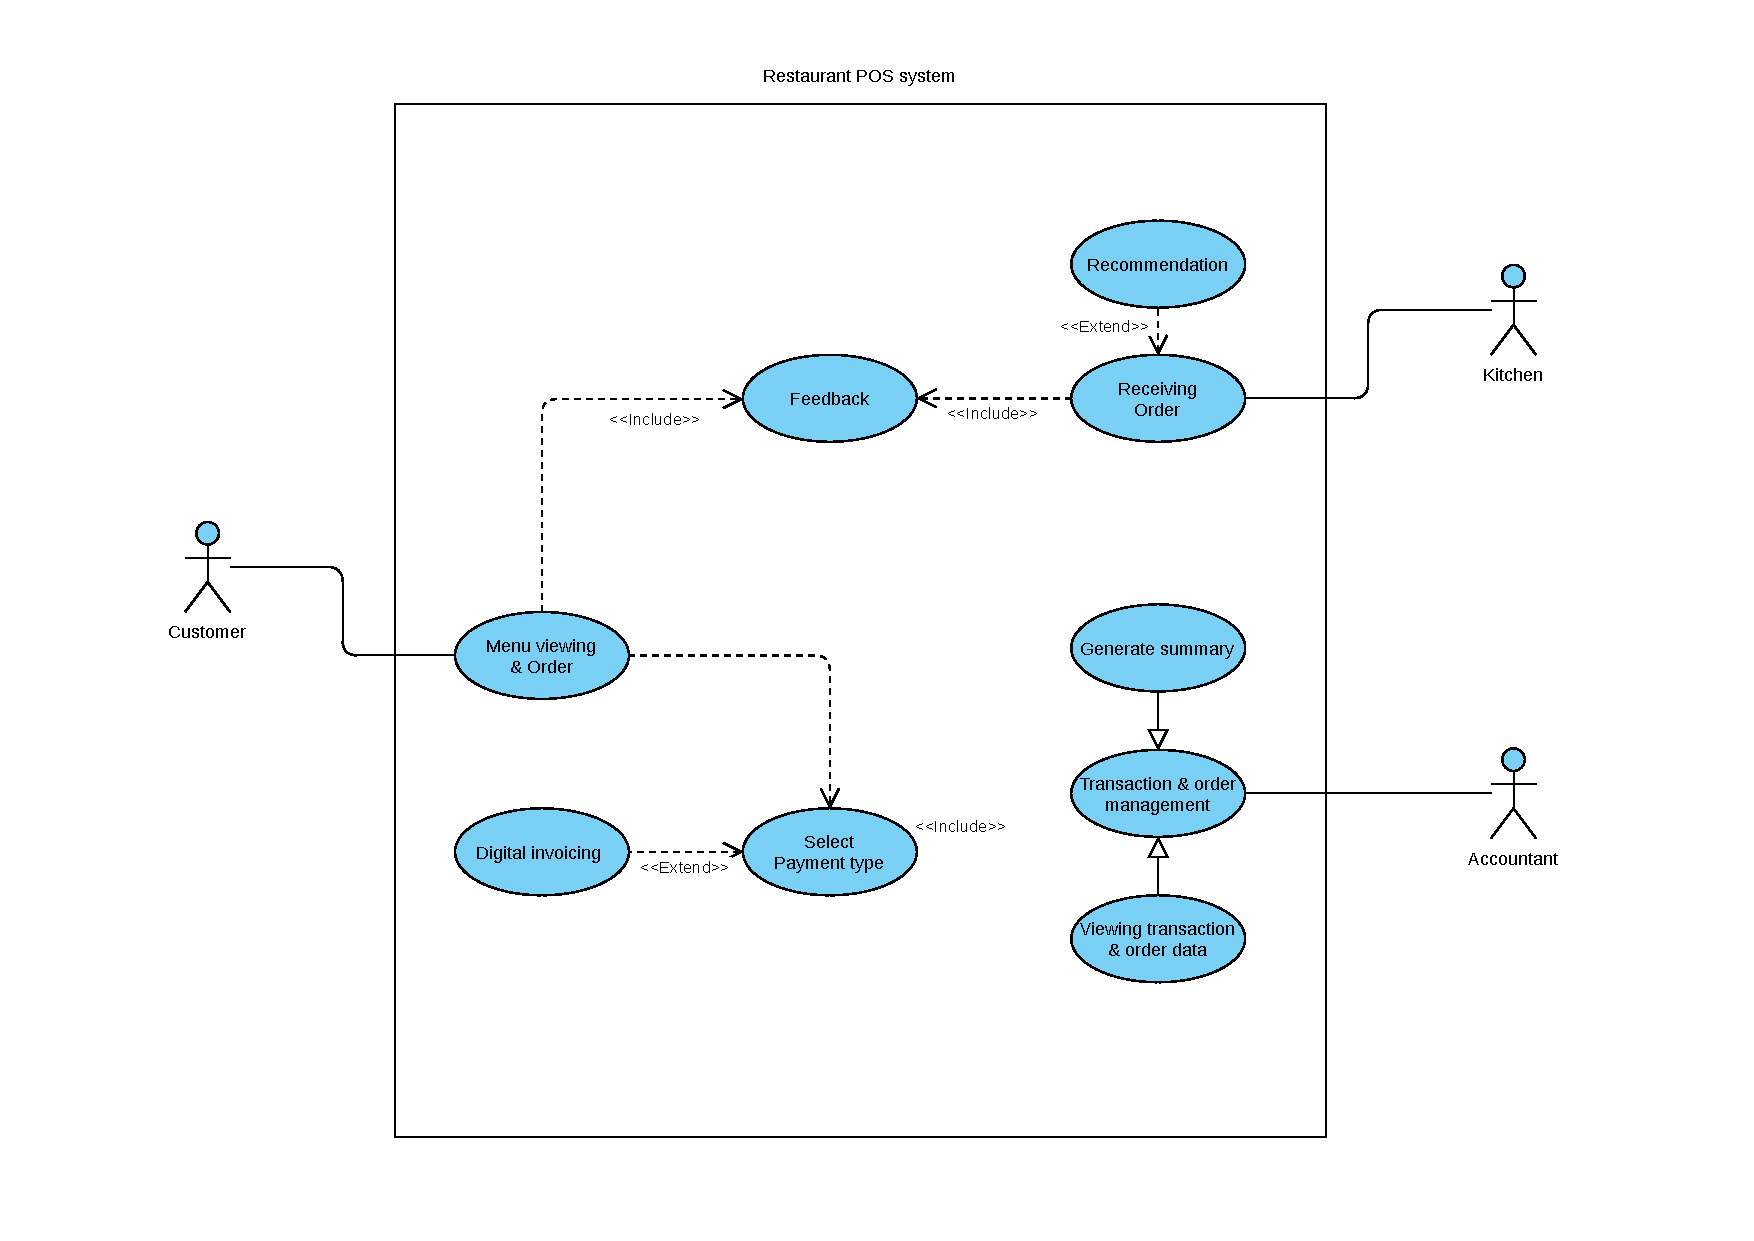
\includegraphics[width=1\textwidth]{general_usecase_diagram.pdf}
    \caption{General use case diagram}
    \label{fig:usecasediagram}
\end{figure}

\subsection{Use case description}
\subsubsection{Menu viewing and ordering}
\begin{usecase}{Menu viewing and ordering}{Customer}
    \addrow{Description}{The customer can view and choose the dishes they want from the menu when they access to the system's customer's side.}
    \addrow{Precondition}{The customer need to access to the system's customer's side through the QR code provided on each table.}
    \addmulrow{Normal flow}{
        \item[1.] Customers go to the menu page by QR code.
        \item[2.] Customers browsing through the menu.
        \item[3.] Customers choose their dishes by tapping or clicking the "Add to order list" button located at the end of each dish's frame.
        \item[4.] After finish choosing their dishes, customers select the "Finish your order" button.
        \item[5.] The order confirming page will appear letting the customer know the status of their dishes.
        \item[6.] All the dishes is available and the confirming page transit to summary of the order, prompting the customer for the payment.}
    \addmulrow{Alternative flow}{
        \item[\emph{Alternative 1.}] At step 5 when the status of dishes changed to "NOT AVAILABLE", the customer will be prompted to choose between changing the dishes or simply removing those dishes by using the provided dialog box.
        \begin{enumerate}[]
            \item[1.1] If the customer want to change the dishes then the customer will be directed to the menu page and started again from step 1.
            \item[1.2] If the customer want to remove the unavailable dishes then the system will proceed to do so.
        \end{enumerate}
        \item[\emph{Alternative 2.}] At the step 5, the customer receive a recommendation from the kitchen. The customer will then be prompted to choose between adding recommended dishes or keeping their order.
        \begin{enumerate}
            \item[2.1] If the customer want to add the dishes then the system will automatically add the dishes to the order.
            \item[2.2] If the customer don't want to change their order then the system will proceed to do so.
        \end{enumerate}
        }
\end{usecase}
\newpage
\subsubsubsection{Customers' main flow}
\begin{figure}[htbp]
    \centering
    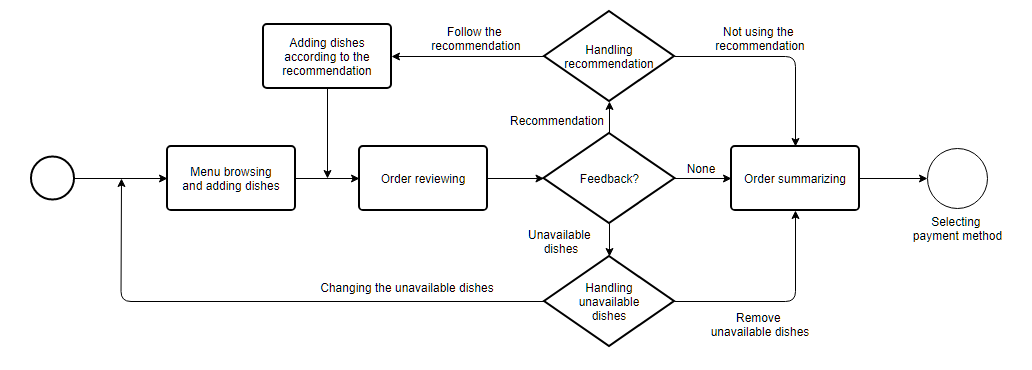
\includegraphics[width=1.0\textwidth]{menu_viewing_ordering.png}
    \caption{Menu viewing and ordering main flow}
    \label{fig:my_label}
\end{figure}
\subsubsubsection{Mockup}
The full mockup will be included at \texttt{Menu\_viewing\_and\_ordering.pdf} file.
\begin{enumerate}[wide=0pt]
    \item Menu Page: \\
    \emph{Description:}  \\
    \begin{tabularx}{\textwidth}{|l|p{0.14\linewidth}|p{0.25\linewidth}|p{0.09\linewidth}|p{0.065\linewidth}|l|X|}
    \hline
    \textbf{No.} & \textbf{Field name} & \textbf{Description} & \textbf{Control type} & \textbf{Data Type} & \textbf{Mandatory} & \textbf{Default value} \\
    \hline
    1. & Check button & To see the ordered dishes and their status & Button & N/A & Yes & N/A \\
    \hline
    2. & Filter & To filter the dishes by specific categories & List of button & N/A & No & N/A \\ 
    \hline
    3. & Dish info card & Display dish's info in a new page & Link box & Text, Image & Yes & N/A \\ 
    \hline
    4. & Add to cart button & Add the dish to the order & Button & N/A & Yes & N/A \\
    \hline
    
    \end{tabularx}
    \begin{figure}[htbp]
            \centering
            
            \resizebox{0.7\textwidth}{!}{%


\tikzset{every picture/.style={line width=0.75pt}} %set default line width to 0.75pt        

\begin{tikzpicture}[x=0.75pt,y=0.75pt,yscale=-1,xscale=1]
%uncomment if require: \path (0,473); %set diagram left start at 0, and has height of 473

%Image [id:dp3126442040850481] 
\draw (254.94,230.84) node  {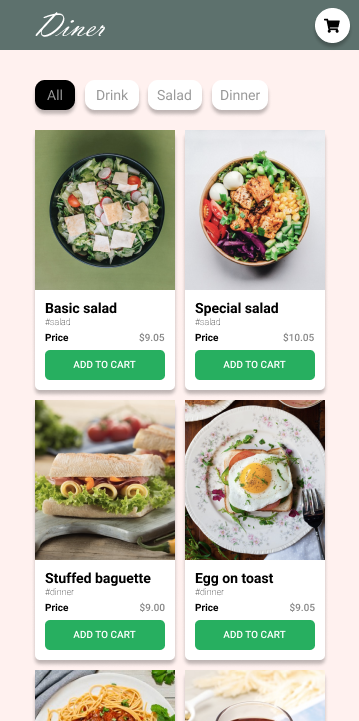
\includegraphics[width=172.41pt,height=346.25pt]{menu_page.png}};
%Straight Lines [id:da08070854781688008] 
\draw [color={rgb, 255:red, 255; green, 0; blue, 0 }  ,draw opacity=1 ]   (390,16) -- (377,16) -- (363,16) ;
\draw [shift={(363,16)}, rotate = 180] [color={rgb, 255:red, 255; green, 0; blue, 0 }  ,draw opacity=1 ][fill={rgb, 255:red, 255; green, 0; blue, 0 }  ,fill opacity=1 ][line width=0.75]      (0, 0) circle [x radius= 3.35, y radius= 3.35]   ;
%Straight Lines [id:da4471527597555851] 
\draw [color={rgb, 255:red, 255; green, 0; blue, 0 }  ,draw opacity=1 ]   (120,60) -- (140,60) -- (164,60) ;
\draw [shift={(164,60)}, rotate = 0] [color={rgb, 255:red, 255; green, 0; blue, 0 }  ,draw opacity=1 ][fill={rgb, 255:red, 255; green, 0; blue, 0 }  ,fill opacity=1 ][line width=0.75]      (0, 0) circle [x radius= 3.35, y radius= 3.35]   ;
%Straight Lines [id:da5179098513663347] 
\draw [color={rgb, 255:red, 255; green, 0; blue, 0 }  ,draw opacity=1 ]   (120,150) -- (140,150) -- (164,150) ;
\draw [shift={(164,150)}, rotate = 0] [color={rgb, 255:red, 255; green, 0; blue, 0 }  ,draw opacity=1 ][fill={rgb, 255:red, 255; green, 0; blue, 0 }  ,fill opacity=1 ][line width=0.75]      (0, 0) circle [x radius= 3.35, y radius= 3.35]   ;
%Straight Lines [id:da8597955221467493] 
\draw [color={rgb, 255:red, 255; green, 0; blue, 0 }  ,draw opacity=1 ]   (120,236) -- (140,236) -- (174,236) ;
\draw [shift={(174,236)}, rotate = 0] [color={rgb, 255:red, 255; green, 0; blue, 0 }  ,draw opacity=1 ][fill={rgb, 255:red, 255; green, 0; blue, 0 }  ,fill opacity=1 ][line width=0.75]      (0, 0) circle [x radius= 3.35, y radius= 3.35]   ;

% Text Node
\draw (391,7) node [anchor=north west][inner sep=0.75pt]  [font=\normalsize,color={rgb, 255:red, 255; green, 0; blue, 0 }  ,opacity=1 ] [align=left] {1.};
% Text Node
\draw (105,51) node [anchor=north west][inner sep=0.75pt]  [font=\normalsize,color={rgb, 255:red, 255; green, 0; blue, 0 }  ,opacity=1 ] [align=left] {2.};
% Text Node
\draw (105,141) node [anchor=north west][inner sep=0.75pt]  [font=\normalsize,color={rgb, 255:red, 255; green, 0; blue, 0 }  ,opacity=1 ] [align=left] {3.};
% Text Node
\draw (104,226) node [anchor=north west][inner sep=0.75pt]  [font=\normalsize,color={rgb, 255:red, 255; green, 0; blue, 0 }  ,opacity=1 ] [align=left] {4.};


\end{tikzpicture}


            }%
            \caption{Mock up 1: Menu page}
            \label{fig:menu}
        \end{figure}
        
    \newpage
    
    \item Dish info page: \\
        \begin{figure}[htbp]
            \centering
            
            \resizebox{0.7\textwidth}{!}{%
                \tikzset{every picture/.style={line width=0.75pt}} %set default line width to 0.75pt        
                \begin{tikzpicture}[x=0.75pt,y=0.75pt,yscale=-1,xscale=1]
                %uncomment if require: \path (0,614); %set diagram left start at 0, and has height of 614
                %Image [id:dp2943344730018669] 
                \draw (254.94,230.84) node  {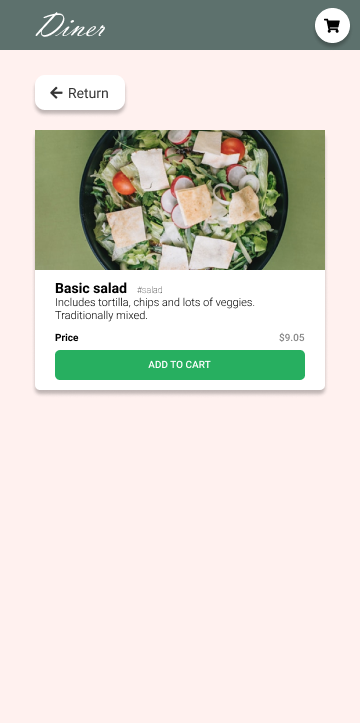
\includegraphics[width=172.41pt,height=346.25pt]{dishinfo_page.png}};
                %Straight Lines [id:da4982441404610163] 
                \draw [color={rgb, 255:red, 255; green, 0; blue, 0 }  ,draw opacity=1 ]   (387,16) -- (374,16) -- (360,16) ;
                \draw [shift={(360,16)}, rotate = 180] [color={rgb, 255:red, 255; green, 0; blue, 0 }  ,draw opacity=1 ][fill={rgb, 255:red, 255; green, 0; blue, 0 }  ,fill opacity=1 ][line width=0.75]      (0, 0) circle [x radius= 3.35, y radius= 3.35]   ;
                %Straight Lines [id:da37852756129422205] 
                \draw [color={rgb, 255:red, 255; green, 0; blue, 0 }  ,draw opacity=1 ]   (117,60) -- (137,60) -- (170,60) ;
                \draw [shift={(170,60)}, rotate = 0] [color={rgb, 255:red, 255; green, 0; blue, 0 }  ,draw opacity=1 ][fill={rgb, 255:red, 255; green, 0; blue, 0 }  ,fill opacity=1 ][line width=0.75]      (0, 0) circle [x radius= 3.35, y radius= 3.35]   ;
                %Straight Lines [id:da380524097945073] 
                \draw [color={rgb, 255:red, 255; green, 0; blue, 0 }  ,draw opacity=1 ]   (117,150) -- (137,150) -- (170,150) ;
                \draw [shift={(170,150)}, rotate = 0] [color={rgb, 255:red, 255; green, 0; blue, 0 }  ,draw opacity=1 ][fill={rgb, 255:red, 255; green, 0; blue, 0 }  ,fill opacity=1 ][line width=0.75]      (0, 0) circle [x radius= 3.35, y radius= 3.35]   ;
                %Straight Lines [id:da4363952196339391] 
                \draw [color={rgb, 255:red, 255; green, 0; blue, 0 }  ,draw opacity=1 ]   (120,230) -- (140,230) -- (190,230) ;
                \draw [shift={(190,230)}, rotate = 0] [color={rgb, 255:red, 255; green, 0; blue, 0 }  ,draw opacity=1 ][fill={rgb, 255:red, 255; green, 0; blue, 0 }  ,fill opacity=1 ][line width=0.75]      (0, 0) circle [x radius= 3.35, y radius= 3.35]   ;
                
                % Text Node
                \draw (388,7) node [anchor=north west][inner sep=0.75pt]  [font=\normalsize,color={rgb, 255:red, 255; green, 0; blue, 0 }  ,opacity=1 ] [align=left] {5.};
                % Text Node
                \draw (102,51) node [anchor=north west][inner sep=0.75pt]  [font=\normalsize,color={rgb, 255:red, 255; green, 0; blue, 0 }  ,opacity=1 ] [align=left] {6.};
                % Text Node
                \draw (102,141) node [anchor=north west][inner sep=0.75pt]  [font=\normalsize,color={rgb, 255:red, 255; green, 0; blue, 0 }  ,opacity=1 ] [align=left] {7.};
                % Text Node
                \draw (101,221) node [anchor=north west][inner sep=0.75pt]  [font=\normalsize,color={rgb, 255:red, 255; green, 0; blue, 0 }  ,opacity=1 ] [align=left] {8.};
                \end{tikzpicture}
            }%
            \caption{Mock up 2: Dish info page}
            \label{fig:dishinfo}
        \end{figure}
    \newpage
    \emph{Description:}  \\
    \begin{tabularx}{\textwidth}{|l|p{0.14\linewidth}|p{0.25\linewidth}|p{0.09\linewidth}|p{0.065\linewidth}|l|X|}
        \hline
        \textbf{No.} & \textbf{Field name} & \textbf{Description} & \textbf{Control type} & \textbf{Data Type} & \textbf{Mandatory} & \textbf{Default value} \\
        \hline
        5. & Check button & To see the ordered dishes and their status & Button & N/A & Yes & N/A \\
        \hline
        6. & Return button & Return to the menu page & Button & N/A & Yes & N/A \\ 
        \hline
        7. & Dish info card & Display detailed dish's info & Box & Text, Image & Yes & N/A \\ 
        \hline
        8. & Add to cart button & Add the dish to the order & Button & N/A & Yes & N/A \\
        \hline
    \end{tabularx} 
    \\
    \item Order review page: \\
    \emph{Description:}  \\
    \begin{tabularx}{\textwidth}{|l|p{0.14\linewidth}|p{0.25\linewidth}|p{0.09\linewidth}|p{0.065\linewidth}|l|X|}
        \hline
        \textbf{No.} & \textbf{Field name} & \textbf{Description} & \textbf{Control type} & \textbf{Data Type} & \textbf{Mandatory} & \textbf{Default value} \\
        \hline
        9. & Next button & To confirm the order and see the order's summary & Button & N/A & Yes & N/A \\
        \hline
        11. & Kebab menu button & To open a menu with "Replace" and "Remove" dish option  & Button & N/A & Yes & N/A \\ 
        \hline
        12. & Dish info card & Display dish's status and allow to change the dish's number of portion & Box & Text, Button & Yes & N/A \\ 
        \hline
        13. & Not available dish field & Prompt the customers to change or remove the unavailable dish & Box & Text, Button & Yes & N/A \\
        \hline
        14. & Recommend dishes field & Prompt the customers if they want to add the recommended dishes or not & Box & Text, Button & Yes & N/A \\
        \hline
    \end{tabularx}
    
        \begin{figure}[htbp]
            \centering
            \resizebox{0.7\textwidth}{!}{%
                \tikzset{every picture/.style={line width=0.75pt}} %set default line width to 0.75pt        
                
                \begin{tikzpicture}[x=0.75pt,y=0.75pt,yscale=-1,xscale=1]
                %uncomment if require: \path (0,500); %set diagram left start at 0, and has height of 500
                
                %Image [id:dp41692429085977345] 
                \draw (254.94,230.84) node  {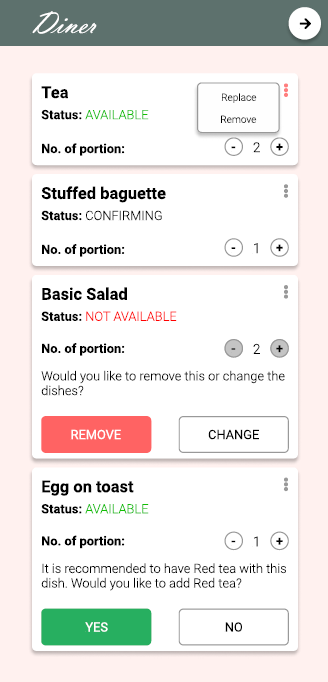
\includegraphics[width=172.41pt,height=346.25pt]{confirming_page.png}};
                %Straight Lines [id:da3098508428933635] 
                \draw [color={rgb, 255:red, 255; green, 0; blue, 0 }  ,draw opacity=1 ]   (387,16) -- (374,16) -- (360,16) ;
                \draw [shift={(360,16)}, rotate = 180] [color={rgb, 255:red, 255; green, 0; blue, 0 }  ,draw opacity=1 ][fill={rgb, 255:red, 255; green, 0; blue, 0 }  ,fill opacity=1 ][line width=0.75]      (0, 0) circle [x radius= 3.35, y radius= 3.35]   ;
                %Straight Lines [id:da7368719099511032] 
                \draw [color={rgb, 255:red, 255; green, 0; blue, 0 }  ,draw opacity=1 ]   (390,60) -- (370,60) -- (343,60) ;
                \draw [shift={(343,60)}, rotate = 180] [color={rgb, 255:red, 255; green, 0; blue, 0 }  ,draw opacity=1 ][fill={rgb, 255:red, 255; green, 0; blue, 0 }  ,fill opacity=1 ][line width=0.75]      (0, 0) circle [x radius= 3.35, y radius= 3.35]   ;
                %Straight Lines [id:da7060081098703315] 
                \draw [color={rgb, 255:red, 255; green, 0; blue, 0 }  ,draw opacity=1 ]   (117,90) -- (137,90) -- (170,90) ;
                \draw [shift={(170,90)}, rotate = 0] [color={rgb, 255:red, 255; green, 0; blue, 0 }  ,draw opacity=1 ][fill={rgb, 255:red, 255; green, 0; blue, 0 }  ,fill opacity=1 ][line width=0.75]      (0, 0) circle [x radius= 3.35, y radius= 3.35]   ;
                %Straight Lines [id:da5663028475363252] 
                \draw [color={rgb, 255:red, 255; green, 0; blue, 0 }  ,draw opacity=1 ]   (120,280) -- (140,280) -- (180,280) ;
                \draw [shift={(180,280)}, rotate = 0] [color={rgb, 255:red, 255; green, 0; blue, 0 }  ,draw opacity=1 ][fill={rgb, 255:red, 255; green, 0; blue, 0 }  ,fill opacity=1 ][line width=0.75]      (0, 0) circle [x radius= 3.35, y radius= 3.35]   ;
                %Straight Lines [id:da7836308850119804] 
                \draw [color={rgb, 255:red, 255; green, 0; blue, 0 }  ,draw opacity=1 ]   (387,36) -- (340,36) -- (330,20) ;
                \draw [shift={(330,20)}, rotate = 237.99] [color={rgb, 255:red, 255; green, 0; blue, 0 }  ,draw opacity=1 ][fill={rgb, 255:red, 255; green, 0; blue, 0 }  ,fill opacity=1 ][line width=0.75]      (0, 0) circle [x radius= 3.35, y radius= 3.35]   ;
                %Straight Lines [id:da5639527194471947] 
                \draw [color={rgb, 255:red, 255; green, 0; blue, 0 }  ,draw opacity=1 ]   (390,410) -- (370,410) -- (333,410) ;
                \draw [shift={(333,410)}, rotate = 180] [color={rgb, 255:red, 255; green, 0; blue, 0 }  ,draw opacity=1 ][fill={rgb, 255:red, 255; green, 0; blue, 0 }  ,fill opacity=1 ][line width=0.75]      (0, 0) circle [x radius= 3.35, y radius= 3.35]   ;
                
                % Text Node
                \draw (388,7) node [anchor=north west][inner sep=0.75pt]  [font=\normalsize,color={rgb, 255:red, 255; green, 0; blue, 0 }  ,opacity=1 ] [align=left] {9.};
                % Text Node
                \draw (391,51) node [anchor=north west][inner sep=0.75pt]  [font=\normalsize,color={rgb, 255:red, 255; green, 0; blue, 0 }  ,opacity=1 ] [align=left] {11.};
                % Text Node
                \draw (96,81) node [anchor=north west][inner sep=0.75pt]  [font=\normalsize,color={rgb, 255:red, 255; green, 0; blue, 0 }  ,opacity=1 ] [align=left] {12.};
                % Text Node
                \draw (99,272) node [anchor=north west][inner sep=0.75pt]  [font=\normalsize,color={rgb, 255:red, 255; green, 0; blue, 0 }  ,opacity=1 ] [align=left] {13.};
                % Text Node
                \draw (388,27) node [anchor=north west][inner sep=0.75pt]  [font=\normalsize,color={rgb, 255:red, 255; green, 0; blue, 0 }  ,opacity=1 ] [align=left] {10.};
                % Text Node
                \draw (391,401) node [anchor=north west][inner sep=0.75pt]  [font=\normalsize,color={rgb, 255:red, 255; green, 0; blue, 0 }  ,opacity=1 ] [align=left] {14.};
                
                
                \end{tikzpicture}
            }%
            \caption{Mock up 3: Order review page}
            \label{fig:reviewing}
        \end{figure}
    \newpage
    \item Dish changing page: \\
    \begin{figure}[htbp]
            \centering
            \resizebox{0.7\textwidth}{!}{%
                \tikzset{every picture/.style={line width=0.75pt}} %set default line width to 0.75pt        
                
                \begin{tikzpicture}[x=0.75pt,y=0.75pt,yscale=-1,xscale=1]
                %uncomment if require: \path (0,627); %set diagram left start at 0, and has height of 627
                
                %Image [id:dp6317308650333988] 
                \draw (254.94,229.16) node  {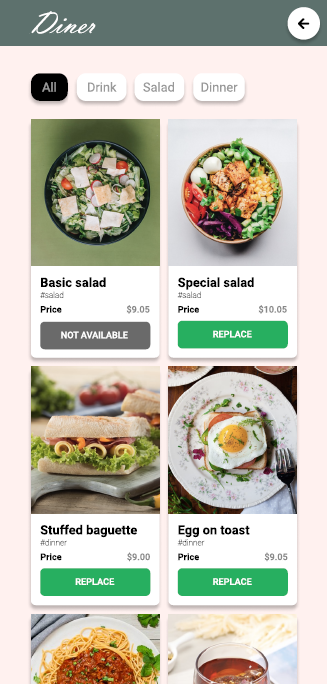
\includegraphics[width=172.41pt,height=346.25pt]{replacing_page.png}};
                %Straight Lines [id:da7705543671147561] 
                \draw [color={rgb, 255:red, 255; green, 0; blue, 0 }  ,draw opacity=1 ]   (390,14.33) -- (377,14.33) -- (363,14.33) ;
                \draw [shift={(363,14.33)}, rotate = 180] [color={rgb, 255:red, 255; green, 0; blue, 0 }  ,draw opacity=1 ][fill={rgb, 255:red, 255; green, 0; blue, 0 }  ,fill opacity=1 ][line width=0.75]      (0, 0) circle [x radius= 3.35, y radius= 3.35]   ;
                %Straight Lines [id:da8027898862374145] 
                \draw [color={rgb, 255:red, 255; green, 0; blue, 0 }  ,draw opacity=1 ]   (120,58.33) -- (137,58.33) -- (161,58.33) ;
                \draw [shift={(161,58.33)}, rotate = 0] [color={rgb, 255:red, 255; green, 0; blue, 0 }  ,draw opacity=1 ][fill={rgb, 255:red, 255; green, 0; blue, 0 }  ,fill opacity=1 ][line width=0.75]      (0, 0) circle [x radius= 3.35, y radius= 3.35]   ;
                %Straight Lines [id:da2738354007738477] 
                \draw [color={rgb, 255:red, 255; green, 0; blue, 0 }  ,draw opacity=1 ]   (390,231.33) -- (357,231.33) -- (325,231.33) ;
                \draw [shift={(325,231.33)}, rotate = 180] [color={rgb, 255:red, 255; green, 0; blue, 0 }  ,draw opacity=1 ][fill={rgb, 255:red, 255; green, 0; blue, 0 }  ,fill opacity=1 ][line width=0.75]      (0, 0) circle [x radius= 3.35, y radius= 3.35]   ;
                
                % Text Node
                \draw (391,5.33) node [anchor=north west][inner sep=0.75pt]  [font=\normalsize,color={rgb, 255:red, 255; green, 0; blue, 0 }  ,opacity=1 ] [align=left] {15.};
                % Text Node
                \draw (100,50.33) node [anchor=north west][inner sep=0.75pt]  [font=\normalsize,color={rgb, 255:red, 255; green, 0; blue, 0 }  ,opacity=1 ] [align=left] {16.};
                % Text Node
                \draw (395,222) node [anchor=north west][inner sep=0.75pt]  [font=\normalsize,color={rgb, 255:red, 255; green, 0; blue, 0 }  ,opacity=1 ] [align=left] {17.};
                
                
                \end{tikzpicture}
            }%
            \caption{Mock up 4: Dish change page}
            \label{fig:changing}
        \end{figure}
        \newpage
    \emph{Description:}  \\
    \begin{tabularx}{\textwidth}{|l|p{0.14\linewidth}|p{0.25\linewidth}|p{0.09\linewidth}|p{0.065\linewidth}|l|X|}
        \hline
        \textbf{No.} & \textbf{Field name} & \textbf{Description} & \textbf{Control type} & \textbf{Data Type} & \textbf{Mandatory} & \textbf{Default value} \\
        \hline
        15. & Back button & To return to the order review page & Button & N/A & Yes & N/A \\
        \hline
        16. & Filter & To filter the dishes by specific categories & List of button & N/A & No & N/A \\ 
        \hline
        17. & Replace button & To replace the dish issued the "Replace" or "Change" command & Button & Button & Yes & N/A \\ 
        \hline
    \end{tabularx} \\
   \item Summary page: \\
    \emph{Description:}  \\
    \begin{tabularx}{\textwidth}{|l|p{0.14\linewidth}|p{0.25\linewidth}|p{0.09\linewidth}|p{0.065\linewidth}|l|X|}
        \hline
        \textbf{No.} & \textbf{Field name} & \textbf{Description} & \textbf{Control type} & \textbf{Data Type} & \textbf{Mandatory} & \textbf{Default value} \\
        \hline
        18. & Dish summary card & Display dishes' summary and total price & Box & Text & Yes & N/A \\
        \hline
        19. & Checkout button & To checkout and enter the select payment method section & Button & N/A & Yes & N/A \\ 
        \hline
    \end{tabularx}
    
        \begin{figure}[htbp]
            \centering
            \resizebox{0.7\textwidth}{!}{%
                \tikzset{every picture/.style={line width=0.75pt}} %set default line width to 0.75pt        
                
                \begin{tikzpicture}[x=0.75pt,y=0.75pt,yscale=-1,xscale=1]
                %uncomment if require: \path (0,627); %set diagram left start at 0, and has height of 627
                
                %Image [id:dp017841253496055476] 
                \draw (254.94,229.16) node  {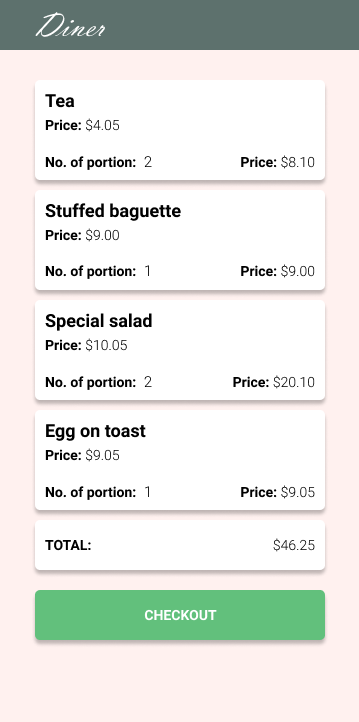
\includegraphics[width=172.41pt,height=346.25pt]{summary_page.png}};
                %Straight Lines [id:da6794045011278274] 
                \draw [color={rgb, 255:red, 255; green, 0; blue, 0 }  ,draw opacity=1 ]   (120,88.33) -- (137,88.33) -- (171,88.33) ;
                \draw [shift={(171,88.33)}, rotate = 0] [color={rgb, 255:red, 255; green, 0; blue, 0 }  ,draw opacity=1 ][fill={rgb, 255:red, 255; green, 0; blue, 0 }  ,fill opacity=1 ][line width=0.75]      (0, 0) circle [x radius= 3.35, y radius= 3.35]   ;
                %Straight Lines [id:da1807773273225548] 
                \draw [color={rgb, 255:red, 255; green, 0; blue, 0 }  ,draw opacity=1 ]   (390,391.33) -- (357,391.33) -- (325,391.33) ;
                \draw [shift={(325,391.33)}, rotate = 180] [color={rgb, 255:red, 255; green, 0; blue, 0 }  ,draw opacity=1 ][fill={rgb, 255:red, 255; green, 0; blue, 0 }  ,fill opacity=1 ][line width=0.75]      (0, 0) circle [x radius= 3.35, y radius= 3.35]   ;
                
                % Text Node
                \draw (100,80.33) node [anchor=north west][inner sep=0.75pt]  [font=\normalsize,color={rgb, 255:red, 255; green, 0; blue, 0 }  ,opacity=1 ] [align=left] {18.};
                % Text Node
                \draw (395,382) node [anchor=north west][inner sep=0.75pt]  [font=\normalsize,color={rgb, 255:red, 255; green, 0; blue, 0 }  ,opacity=1 ] [align=left] {19.};
                
                
                \end{tikzpicture}
            }%
            \caption{Mock up 5: Summary page}
            \label{fig:summary}
        \end{figure}
    \newpage
\end{enumerate}

\newpage
\subsubsection{Order Processing}
\begin{usecase}{Order processing}{Kitchen and Restaurant's staff}
    \addrow{Description}{The kitchen and restaurant's staff can manage all order information from the customers. }
    \addrow{Precondition}{}
    \addmulrow{Normal flow}{
        \item[1.] tbd
    }
    \addmulrow{Alternative flow}{
        \item[\emph{Alternative 1.}] tbd
        }
\end{usecase}
\newpage
%%%%%%%%%%%%%%%%%%%%%%%%%%%%%%%%%

%%%%%%%%%%%%%%%%%%%%%%%%%%%%%%%%%
\section{Non-functional requirements}

\subsection{Product requirements:}
\subsubsection{Performance requirements:}
\begin{itemize}[wide=0pt]
    \item[-] The system should be able to handle at least 300 transactions per day.
    \item[-] The order confirming time (from when the order is sent from the customer to when the kitchen approve its availability) should less than 5 minutes.
    \item[-] The transaction time should not exceed 2 minutes.
    \item[-] The system should be able to handle at least 5 simultaneously table orders.
    \item[-] The rendering time of the system's customer's side should not exceed 3 seconds.
\end{itemize}
\subsubsection{Security Requirements:}
\begin{itemize}[wide=0pt]
    \item[-] All the transaction data should be secured and only allow to read, so that it’s protected from mischievous behaviours and also from internal attack.
    \item[-] The customer's audit information should not be recorded or used from internal sources.
\end{itemize}
\subsubsection{Usability requirements:}
\begin{itemize}[wide=0pt]
    \item[-] The system should be functional on widely used browsers (Chrome, Safari, Firefox, Samsung Internet, Edge, Opera, UC Browser).
    \item[-] The system should be available on usual working hours (from 8 a.m. to 10 p.m.). Downtime within working period shall not exceed 10 seconds in any one day.
    \item[-] The customer should be able to use the system without going through any training.
\end{itemize}

\subsection{Organizational requirements:}
\subsubsection{Operational requirements:}
\begin{itemize}[wide=0pt]
    \item[-] The system should be able to create non-direct interaction between the restaurant's staffs and the customers.
    \item[-] The customers only allow to access the customer-side system using the QR code and password provided on each restaurant's table.
    \item[-] The restaurant's staffs access to the system side using their provided ID.
\end{itemize}

\subsection{External requirements:}
\subsubsection{Legislative requirements:}
\begin{itemize}[wide=0pt]
    \item[-] The invoice and information recording shall be implemented as set out in \emph{Luat Giao dich dien tu 2005}.
\end{itemize}
%%%%%%%%%%%%%%%%%%%%%%%%%%%%%%%%%
\end{document}   